\documentclass[12pt,letterpaper]{article}
\usepackage{graphicx,textcomp}
\usepackage{natbib}
\usepackage{setspace}
\usepackage{fullpage}
\usepackage{color}
\usepackage[reqno]{amsmath}
\usepackage{amsthm}
\usepackage{fancyvrb}
\usepackage{amssymb,enumerate}
\usepackage[all]{xy}
\usepackage{endnotes}
\usepackage{lscape}
\newtheorem{com}{Comment}
\usepackage{float}
\usepackage{hyperref}
\newtheorem{lem} {Lemma}
\newtheorem{prop}{Proposition}
\newtheorem{thm}{Theorem}
\newtheorem{defn}{Definition}
\newtheorem{cor}{Corollary}
\newtheorem{obs}{Observation}
\usepackage[compact]{titlesec}
\usepackage{dcolumn}
\usepackage{tikz}
\usetikzlibrary{arrows}
\usepackage{multirow}
\usepackage{xcolor}
\newcolumntype{.}{D{.}{.}{-1}}
\newcolumntype{d}[1]{D{.}{.}{#1}}
\definecolor{light-gray}{gray}{0.65}
\usepackage{url}
\usepackage{listings}
\usepackage{color}

\definecolor{codegreen}{rgb}{0,0.6,0}
\definecolor{codegray}{rgb}{0.5,0.5,0.5}
\definecolor{codepurple}{rgb}{0.58,0,0.82}
\definecolor{backcolour}{rgb}{0.95,0.95,0.92}

\lstdefinestyle{mystyle}{
	backgroundcolor=\color{backcolour},   
	commentstyle=\color{codegreen},
	keywordstyle=\color{magenta},
	numberstyle=\tiny\color{codegray},
	stringstyle=\color{codepurple},
	basicstyle=\footnotesize,
	breakatwhitespace=false,         
	breaklines=true,                 
	captionpos=b,                    
	keepspaces=true,                 
	numbers=left,                    
	numbersep=5pt,                  
	showspaces=false,                
	showstringspaces=false,
	showtabs=false,                  
	tabsize=2
}
\lstset{style=mystyle}
\newcommand{\Sref}[1]{Section~\ref{#1}}
\newtheorem{hyp}{Hypothesis}

\title{Problem Set 3}
\date{Due: November 19, 2022}
\author{Jacqueline Bouvier Applied Stats/Quant Methods 1}

\begin{document}
	\maketitle
	\section*{Instructions}
	\begin{itemize}
		\item Please show your work! You may lose points by simply writing in the answer. If the problem requires you to execute commands in \texttt{R}, please include the code you used to get your answers. Please also include the \texttt{.R} file that contains your code. If you are not sure if work needs to be shown for a particular problem, please ask.
	\item Your homework should be submitted electronically on GitHub.
	\item This problem set is due before 23:59 on Sunday November 19, 2023. No late assignments will be accepted.

	\end{itemize}

		\vspace{.25cm}
	
\noindent In this problem set, you will run several regressions and create an add variable plot (see the lecture slides) in \texttt{R} using the \texttt{incumbents\_subset.csv} dataset. Include all of your code.

	\vspace{.5cm}
\section*{Question 1}
\vspace{.25cm}
\noindent We are interested in knowing how the difference in campaign spending between incumbent and challenger affects the incumbent's vote share. 
	\begin{enumerate}
		\item Run a regression where the outcome variable is \texttt{voteshare} and the explanatory variable is \texttt{difflog}.	\vspace{7cm}
\begin{table}[!htbp] \centering   \caption{Vote Share vs Spending Difference}   \label{} \begin{tabular}{@{\extracolsep{5pt}}lc} \\[-1.8ex]\hline \hline \\[-1.8ex]  & \multicolumn{1}{c}{\textit{Dependent variable:}} \\ \cline{2-2} \\[-1.8ex] & voteshare \\ \hline \\[-1.8ex]  difflog & 0.042$^{***}$ \\   & (0.001) \\   & \\  Constant & 0.579$^{***}$ \\   & (0.002) \\   & \\ \hline \\[-1.8ex] Observations & 3,193 \\ R$^{2}$ & 0.367 \\ Adjusted R$^{2}$ & 0.367 \\ Residual Std. Error & 0.079 (df = 3191) \\ F Statistic & 1,852.791$^{***}$ (df = 1; 3191) \\ \hline \hline \\[-1.8ex] \textit{Note:}  & \multicolumn{1}{r}{$^{*}$p$<$0.1; $^{**}$p$<$0.05; $^{***}$p$<$0.01} \\ \end{tabular} \end{table} 
	
	
		\item Make a scatterplot of the two variables and add the regression line. 	\vspace{.7cm}
	
		\lstinputlisting[language=R, firstline=42, lastline=45]{PS03_JB.R}]
		Please see Figure 1
	
		\item Save the residuals of the model in a separate object.		\vspace{.7cm}
		\lstinputlisting[language=R, firstline=49, lastline=50]{PS03_JB.R}]
	
		\item Write the prediction equation.
		
		 y = 0.579+0.0417x 	
		 A one unit increase in difflog means a 0.0417 increase in vote share
		
	\end{enumerate}
	
\newpage

\section*{Question 2}
\noindent We are interested in knowing how the difference between incumbent and challenger's spending and the vote share of the presidential candidate of the incumbent's party are related.	\vspace{.25cm}
	\begin{enumerate}
		\item Run a regression where the outcome variable is \texttt{presvote} and the explanatory variable is \texttt{difflog}.	
		\begin{table}[!htbp] \centering   \caption{Pres Vote vs Spending Difference}   \label{} \begin{tabular}{@{\extracolsep{5pt}}lc} \\[-1.8ex]\hline \hline \\[-1.8ex]  & \multicolumn{1}{c}{\textit{Dependent variable:}} \\ \cline{2-2} \\[-1.8ex] & presvote \\ \hline \\[-1.8ex]  difflog & 0.024$^{***}$ \\   & (0.001) \\   & \\  Constant & 0.508$^{***}$ \\   & (0.003) \\   & \\ \hline \\[-1.8ex] Observations & 3,193 \\ R$^{2}$ & 0.088 \\ Adjusted R$^{2}$ & 0.088 \\ Residual Std. Error & 0.110 (df = 3191) \\ F Statistic & 307.715$^{***}$ (df = 1; 3191) \\ \hline \hline \\[-1.8ex] \textit{Note:}  & \multicolumn{1}{r}{$^{*}$p$<$0.1; $^{**}$p$<$0.05; $^{***}$p$<$0.01} \\ \end{tabular} \end{table} 
		\item Make a scatterplot of the two variables and add the regression line. 	
		\lstinputlisting[language=R, firstline=59, lastline=62]{PS03_JB.R}]
		Please see Figure 2
		\item Save the residuals of the model in a separate object.	
			\lstinputlisting[language=R, firstline=65, lastline=66]{PS03_JB.R}]
		\item Write the prediction equation.
		
		y= 0.508+0.024x
		A one unit increase in difflog is a 0.024 unit in Pres Vote
		
	\end{enumerate}
	
	\newpage	
\section*{Question 3}

\noindent We are interested in knowing how the vote share of the presidential candidate of the incumbent's party is associated with the incumbent's electoral success.
	\vspace{.25cm}
	\begin{enumerate}
		\item Run a regression where the outcome variable is \texttt{voteshare} and the explanatory variable is \texttt{presvote}.

			\begin{table}[!htbp] \centering   \caption{Vote Share vs Pres Vote}   \label{} \begin{tabular}{@{\extracolsep{5pt}}lc} \\[-1.8ex]\hline \hline \\[-1.8ex]  & \multicolumn{1}{c}{\textit{Dependent variable:}} \\ \cline{2-2} \\[-1.8ex] & voteshare \\ \hline \\[-1.8ex]  presvote & 0.388$^{***}$ \\   & (0.013) \\   & \\  Constant & 0.441$^{***}$ \\   & (0.008) \\   & \\ \hline \\[-1.8ex] Observations & 3,193 \\ R$^{2}$ & 0.206 \\ Adjusted R$^{2}$ & 0.206 \\ Residual Std. Error & 0.088 (df = 3191) \\ F Statistic & 826.950$^{***}$ (df = 1; 3191) \\ \hline \hline \\[-1.8ex] \textit{Note:}  & \multicolumn{1}{r}{$^{*}$p$<$0.1; $^{**}$p$<$0.05; $^{***}$p$<$0.01} \\ \end{tabular} \end{table} 
		\item Make a scatterplot of the two variables and add the regression line. 

			\lstinputlisting[language=R, firstline=77, lastline=80]{PS03_JB.R}]
			Please see Figure 3
		\item Write the prediction equation.
		
		y= 0.441+0.388x
		A one unit increase in Pres Vote is a 0.388 increase in Vote Share
		
	\end{enumerate}
	

\newpage	
\section*{Question 4}
\noindent The residuals from part (a) tell us how much of the variation in \texttt{voteshare} is $not$ explained by the difference in spending between incumbent and challenger. The residuals in part (b) tell us how much of the variation in \texttt{presvote} is $not$ explained by the difference in spending between incumbent and challenger in the district.
	\begin{enumerate}
		\item Run a regression where the outcome variable is the residuals from Question 1 and the explanatory variable is the residuals from Question 2.	
		\begin{table}[!htbp] \centering   \caption{Vote Share vs Spending Difference}   \label{} \begin{tabular}{@{\extracolsep{5pt}}lc} \\[-1.8ex]\hline \hline \\[-1.8ex]  & \multicolumn{1}{c}{\textit{Dependent variable:}} \\ \cline{2-2} \\[-1.8ex] & resid\_1 \\ \hline \\[-1.8ex]  resid\_2 & 0.257$^{***}$ \\   & (0.012) \\   & \\  Constant & $-$0.000 \\   & (0.001) \\   & \\ \hline \\[-1.8ex] Observations & 3,193 \\ R$^{2}$ & 0.130 \\ Adjusted R$^{2}$ & 0.130 \\ Residual Std. Error & 0.073 (df = 3191) \\ F Statistic & 476.975$^{***}$ (df = 1; 3191) \\ \hline \hline \\[-1.8ex] \textit{Note:}  & \multicolumn{1}{r}{$^{*}$p$<$0.1; $^{**}$p$<$0.05; $^{***}$p$<$0.01} \\ \end{tabular} \end{table} 
		
		\item Make a scatterplot of the two residuals and add the regression line. 	
		\lstinputlisting[language=R, firstline=94, lastline=99]{PS03_JB.R}]
		Please see Figure 4
		\item Write the prediction equation.
		
		y= 2.569e-01x-1.942e-18
		A one unit decrease in the Residuals from residual of question 1 means a decrease of 1.942e-18 of the residuals of question 2
		
	\end{enumerate}
	
	\newpage	

\section*{Question 5}
\noindent What if the incumbent's vote share is affected by both the president's popularity and the difference in spending between incumbent and challenger? 
	\begin{enumerate}
		\item Run a regression where the outcome variable is the incumbent's \texttt{voteshare} and the explanatory variables are \texttt{difflog} and \texttt{presvote}.	
	\begin{table}[!htbp] \centering   \caption{Comparing Difflog and Pres Vote to Vote Share}   \label{} \begin{tabular}{@{\extracolsep{5pt}}lc} \\[-1.8ex]\hline \hline \\[-1.8ex]  & \multicolumn{1}{c}{\textit{Dependent variable:}} \\ \cline{2-2} \\[-1.8ex] & voteshare \\ \hline \\[-1.8ex]  difflog & 0.036$^{***}$ \\   & (0.001) \\   & \\  presvote & 0.257$^{***}$ \\   & (0.012) \\   & \\  Constant & 0.449$^{***}$ \\   & (0.006) \\   & \\ \hline \\[-1.8ex] Observations & 3,193 \\ R$^{2}$ & 0.450 \\ Adjusted R$^{2}$ & 0.449 \\ Residual Std. Error & 0.073 (df = 3190) \\ F Statistic & 1,302.947$^{***}$ (df = 2; 3190) \\ \hline \hline \\[-1.8ex] \textit{Note:}  & \multicolumn{1}{r}{$^{*}$p$<$0.1; $^{**}$p$<$0.05; $^{***}$p$<$0.01} \\ \end{tabular} \end{table} 
		\item Write the prediction equation.	\vspace{6cm}
		
		y= 0.449+0.035x+0.257x1
		For every increase of one unit of difflog and pres vote we would see a 0.035 in vote share along with a 0.257 increase of vote share to the regression lines of the respective explanatory variable.
		
		\item What is it in this output that is identical to the output in Question 4? Why do you think this is the case? \vspace{7cm}
		
		We can see that the standard error residuals are very close to being the same. This could mean that a few different things. Since the residuals are relatively close we could assume that the line of best fit would be similar. The standard error of residuals is from the residuals from question 1 and 2, which then could mean that the data from these two regressions are connected with the multiregression of difflog and pres vote to vote share.
		All the data isn’t equal but highly correlated with each other. We could assume that the data all follows a particular pattern leading to a possible agreement of accepting the hypothesis. 
		
		
		
	\end{enumerate}

\vspace{7cm}






\vspace{.5cm}
	\begin{figure}
	\caption{\footnotesize Figures 1 to 4}
	\label{`Figures'}
	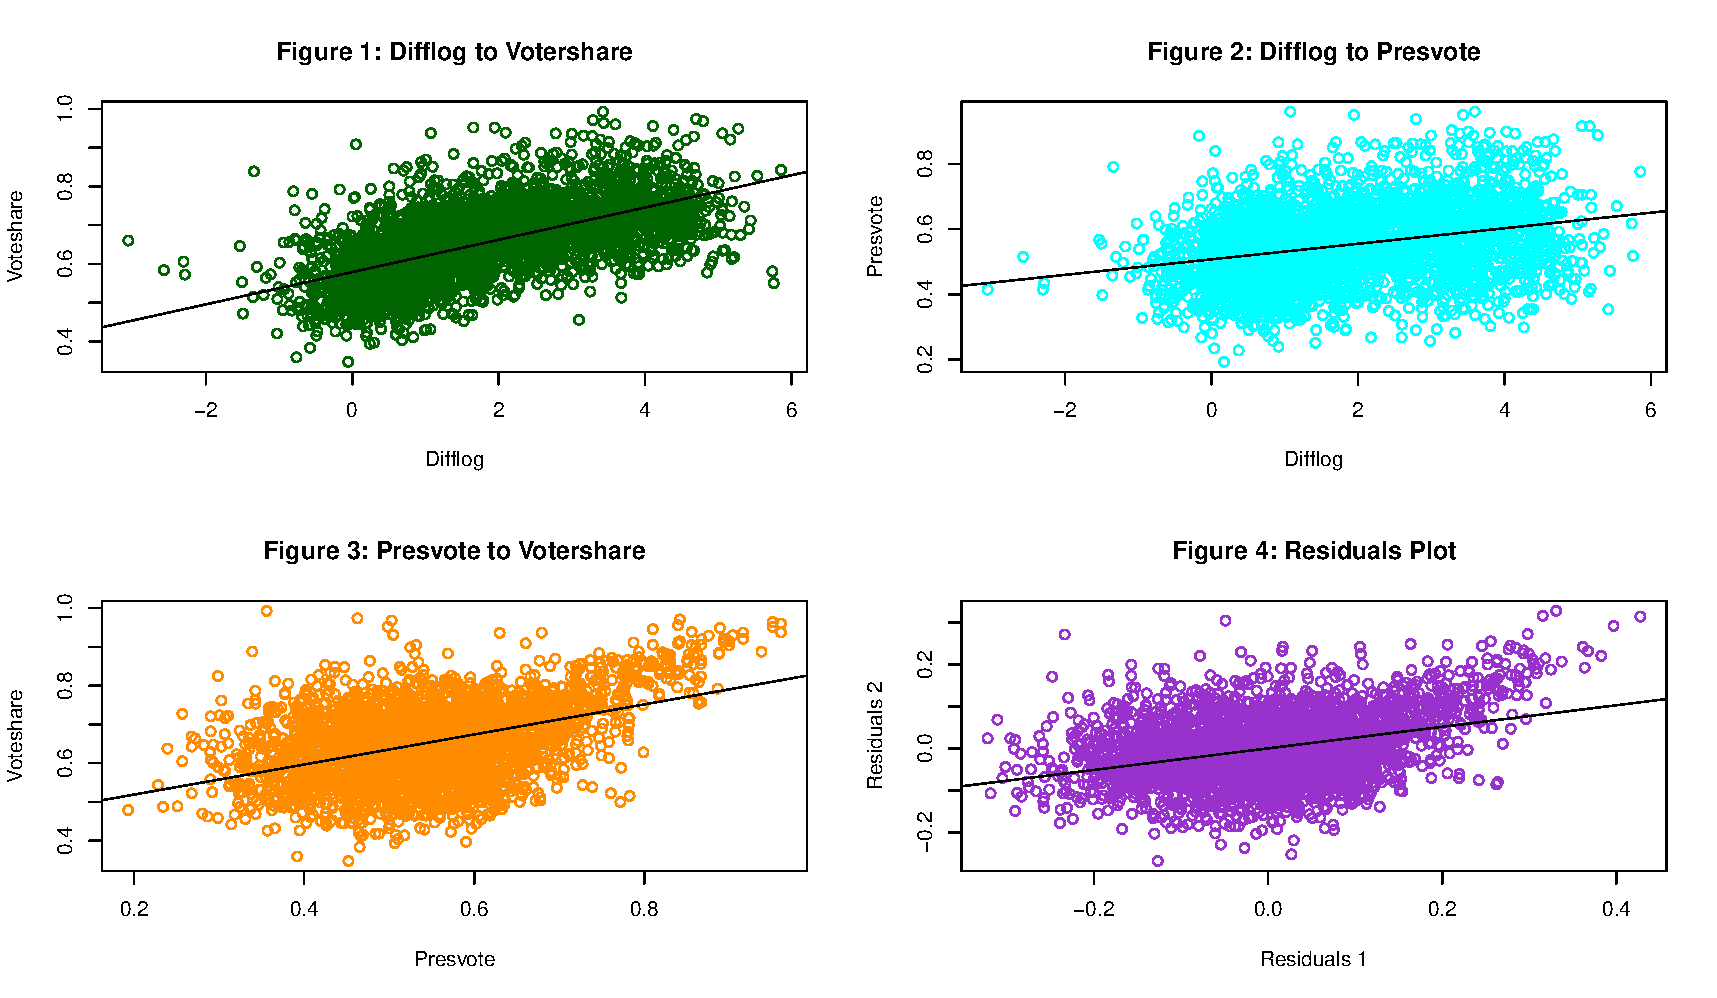
\includegraphics[width=.85\textwidth]{PS03_plots1to4.pdf}
	\centering
\end{figure}
\end{document}
